% Chapter Template

\chapter{Étude bibliographiques} % Main chapter title

\label{ChapterX} % Change X to a consecutive number; for referencing this chapter elsewhere, use \ref{ChapterX}

%----------------------------------------------------------------------------------------
%	SECTION 1
%----------------------------------------------------------------------------------------

\section{Introduction}
Le domaine de l’image numérique est un domaine en pleine expansion. Depuis quelques années, avec l’explosion d’Internet et aussi le développement à grande échelle de la photographie
numérique de haute qualité que nous observons ces dernières années, ce
qui a conduit à un développement constant des bases de données d’images. Le contenu de ces images peut être décrit à deux niveaux différents: 
\begin{itemize}
	\item Au niveau numérique, une image contient des pixels colorés dont on peut extraire des descripteurs de couleurs, des textures et des formes. 
	\item Au niveau sémantique, une image peut être interprétée et peut avoir au moins un sens. 
\end{itemize}

Malheureusement, dans les systèmes d'information d'aujourd'hui, les images sont décrites numériquement alors que les utilisateurs s'intéressent à leur contenu sémantique, il est actuellement difficile de trouver des correspondances entre le niveau numérique et le niveau sémantique. Alors, l’utilisation et la
gestion de ces bases d’images d’une manière efficace est très problématique, elle nécessite de nouvelles techniques de manipulation et de traitement des données. Dans ce contexte, la recherche d’images par le contenu s’intéresse à découvrir des connaissances implicitement contenues dans un ensemble de données en s’appuyant sur différentes approches qui peuvent être mises en œuvre
indépendamment ou couplées. Ces techniques visent à explorer et à décrire le contenu des données, et à en extraire l’information la plus importante et la plus significativement pertinente.
\\

Bien que plusieurs années de travaux scientifiques en recherche d’images par le contenu, ont d’ores et déjà permis la réalisation et le développement des systèmes performants, permettant plusieurs formes et techniques d’indexation par analyse du contenu, mais ce domaine demeure encore aujourd’hui un sujet très ouvert et actif dans la communauté internationale depuis plus d’une dizaine d'années.
\\

L'objectif de ce chapitre est de présenter le principe général des systèmes CBIR. Puis nous nous intéresserons à l'étude des descripteurs et les mesures de similarités les plus utilisés dans l’objectif d’avoir une idée sur quelques approches existantes dans la littérature. 


%-----------------------------------
%	SECTION 1
%-----------------------------------

\section{Représentation machine du contenu visuel des images}

Avant d’entrer dans le sujet proprement dit, il est important de comprendre la nature des objets que nous allons manipuler. Intéressons-nous à la notion d’image, qu’est-ce qu’une image ?

Une des plus anciennes définitions de l'image est celle donnée par Platon [Platon] : « J'appelle image d'abord les ombres ensuite les reflets qu'on voit dans les eaux, ou à la surface des corps opaques, polis et brillants et toutes les représentations de ce genre ». En informatique, une image est une représentation numérique en mémoire d’un sujet imprimé sur une rétine artificielle (matricielle comme le capteur d’un appareil photographique numérique
ou la scène virtuelle d’une image de synthèse ou bien linéaire comme le capteur optique du télécopieur, du photocopieur ou du scanner). \\

On distingue deux types d’images à la composition et au comportement différent: images matricielles et les images vectorielles.

\subsection{Images matricielles (ou images bitmap)}
Les images matricielles sont des images numériques qui stockent les informations sous la forme d’une matrice, des points à plusieurs dimensions, chaque dimension représentant une dimension spatiale (hauteur, largeur), ou autre (niveau de résolution). Dans le cas des images à deux dimensions, les points sont appelés pixels. Elles peuvent être regroupées en plusieurs catégories: images à niveaux de gris, image couleur, image stéréoscopiques et image multicomposante.


\begin{figure}[H]
	\centering
	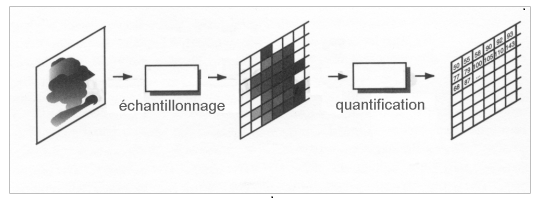
\includegraphics[width=0.6\textwidth]{Figures/imgnum} 
	\caption{Image numérique dont une portion est très agrandie: notion de pixel.}
\end{figure}


Un pixel $(i, j)$, ( i est l’indice de la ligne et j est l’indice de la colonne), possède une valeur $I(i, j)$ qui peut être un scalaire représentant la valeur du niveau de gris du pixel (dans le cas des images noir et blanc ou des images en niveaux de gris), ou un vecteur représentant les trois canaux de la couleur du pixel (dans le cas des images couleurs).

\begin{figure}[H]
	\centering
	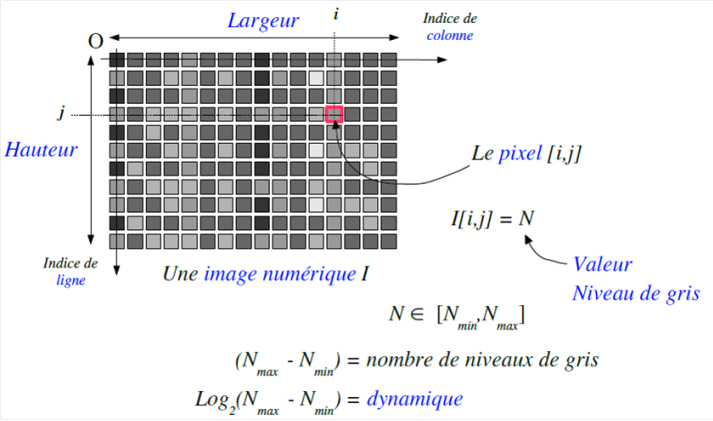
\includegraphics[width=0.6\textwidth]{Figures/pixel} 
	\caption{Image numérique au niveaux de gris: notion de pixel.}
\end{figure}

%-----------------------------------
%	SUBSECTION 1
%-----------------------------------



\subsubsection{Image à niveaux de gris}

Une image numérique à niveaux de gris est une matrice $N \times M$ de pixels. Nous notons $N$ le nombre de lignes et $M$ le nombre de colonnes de l'image. Les images à niveaux de gris sont composées de pixels de valeurs scalaires représentant la luminosité/intensité. En général ces valeurs des pixels sont  codés sur $n$ bits, ce qui lui confère des valeurs entières comprises entre 0 (noir) et $2^n-1$ (blanc), 0 et 255 si $n = 8$. Dans ce cas, le pixel est codé sur un octet (nous disposerons ainsi de $2^8=256$ couleurs). La valeur 255 correspond au blanc, et la valeur 0 correspond au noir. Les valeurs intermédiaires correspondent à des niveaux de gris allant du noir au blanc.\\

La figure ci-dessous montre un sous-tableau de $5 \times 5$ pixels extrait d’une image. Nous pouvons voir les valeurs qui composent le tableau et les niveaux de gris qui permettent d’afficher l’image.

\begin{figure}[H]
	\centering
	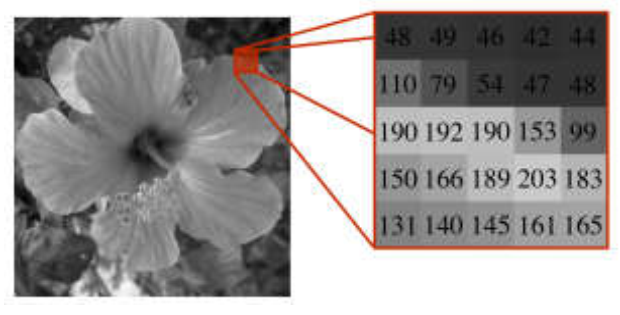
\includegraphics[width=0.4\textwidth]{Figures/gray} 
	\caption{Image à niveaux de gris.}
\end{figure}

%-----------------------------------
%	SUBSECTION 1
%-----------------------------------

\subsubsection{Image couleur}
Une image couleur est composée de pixels dont les valeurs sont en général multicomposantes. \\

En effet, nous pouvons citer parmi les formats les plus utilisés pour représenter la valeur du pixel, le triplet (R,V, B) ou (R,G,B) où R, G et B sont respectivement les valeurs des composantes rouge, verte et bleu du pixel. Chaque composante du triplet est représentée par un entier variant entre 0
(absence de la composante) et 255 (intensité maximale). 

\begin{figure}[H]
	\centering
	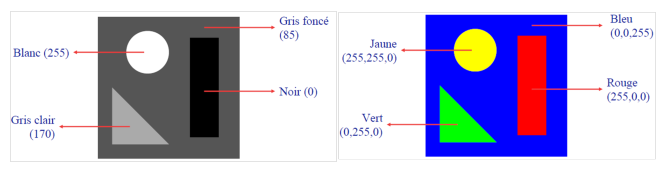
\includegraphics[width=0.6\textwidth]{Figures/grayvscol} 
	\caption{Image à niveaux de gris VS Image couleur.}
\end{figure}

Le triplet (0, 0, 0) correspond au noir, (255, 0, 0) au rouge, (255, 255, 0) au jaune et (255, 255, 255) au blanc. 
Dans ce cas, le pixel est codé sur trois octets. Une image couleur RVB ou (RGB) possède trois composantes tandis qu'une image en niveaux de gris n’en possède qu’une seule. En d'autre termes, Une image couleur correspond à la synthèse additive de 3 images, rouge, vert et bleu. Chaque pixel est donc codé sur $3 \times n = 24 $ bits.

\begin{figure}[H]
	\centering
	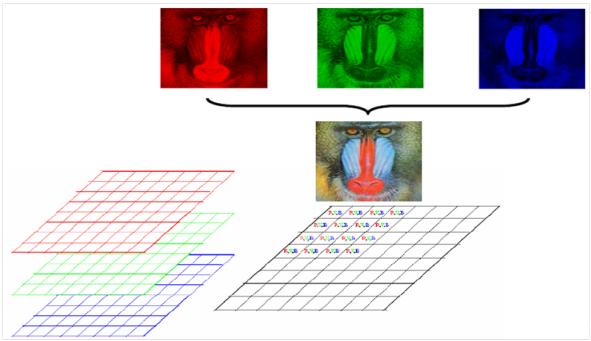
\includegraphics[width=0.4\textwidth]{Figures/rgb} 
	\caption{Image couleur dans l’espace RGB.}
\end{figure}

\subsection{Images vectorielles}

Les images vectorielles, contrairement aux images matricielles, contiennent les primitives de dessin (formes, position, couleurs...) des objets géométriques qu’elles représentent (segments de droite, polygones, arcs de cercles...). Ces images sont essentiellement utilisées pour réaliser des schémas ou des plans. Leur codage dépend directement du logiciel qui a permis de les créer. Ces images présentent deux avantages: elles occupent peu de place en mémoire et peuvent être facilement redimensionnées sans perte d'information.

\begin{figure}[H]
	\centering
	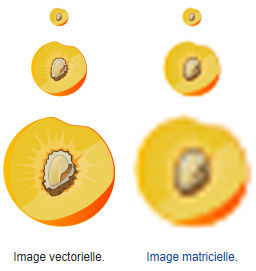
\includegraphics[width=0.4\textwidth]{Figures/vecteur} 
	\caption{Une image vectorielle: redimensionnable sans perte de qualité, contrairement à une image matricielle.}
\end{figure}



%-----------------------------------
%	SECTION 2
%-----------------------------------

\section{Systèmes de recherche d’image par contenu (CBIR)}
Les chercheurs dans le domaine de la vision par ordinateur se posent le problème de l'indexation automatique des images par leur contenu, qui permet la recherche dimages par le
contenu (CBIR).\\

CBIR (Content Based Image Retrieval) est un système qui utilise des contenus visuels pour récupérer des images à partir d'une base de données d'images. Ce système est devenu indispensable parce qu'il peut effectivement surmonter les problèmes d'un TBIR (Text Based Image Retrieval). Dans le CBIR, le contenu visuel est extrait par plusieurs techniques:
histogramme, segmentation... Il est également décrit par le vecteur de caractéristiques multidimensionnel. La performance du système de recherche d'images basées sur le contenu est principalement influencée par la qualité et la pertinence du vecteur de caractéristiques et la mesures de similarité. \\

Le CBIR diffère de la recherche d’information textuelle essentiellement par le fait que les bases de données d’images sont non-structurées, les images numériques n’étant que des matrices
d’intensités de pixels, sans signification inhérente les unes par rapport aux autres. Donc avant même de commencer à faire des hypothèses sur le contenu de l’image, une des questions clé dans tout type de traitement d’image est l’extraction de l’information utile à partir de ces matrices de pixels \textbf{[Quel08]}.\\

Le principe général de la recherche d'image par le contenu comporte deux étapes:
\begin{itemize}
	\item  Lors d'une première phase hors ligne (étape d'indexation), on calcule les descripteurs des images et on les stocke dans une base de données appelé base des indix.
	\item La seconde phase, dite de recherche se déroule en ligne. L'utilisateur soumet une image comme requête. Le système calcule le descripteur selon le même mode que lors de la première phase d'indexation. Ainsi, ce descripteur est comparé à l'ensemble des descripteurs préalablement stockés dans la base d'index pour en ramener les images les plus semblables à la requête.
\end{itemize}

\begin{figure}[H]
	    \label{fig:cbir_principe}
		\centering
		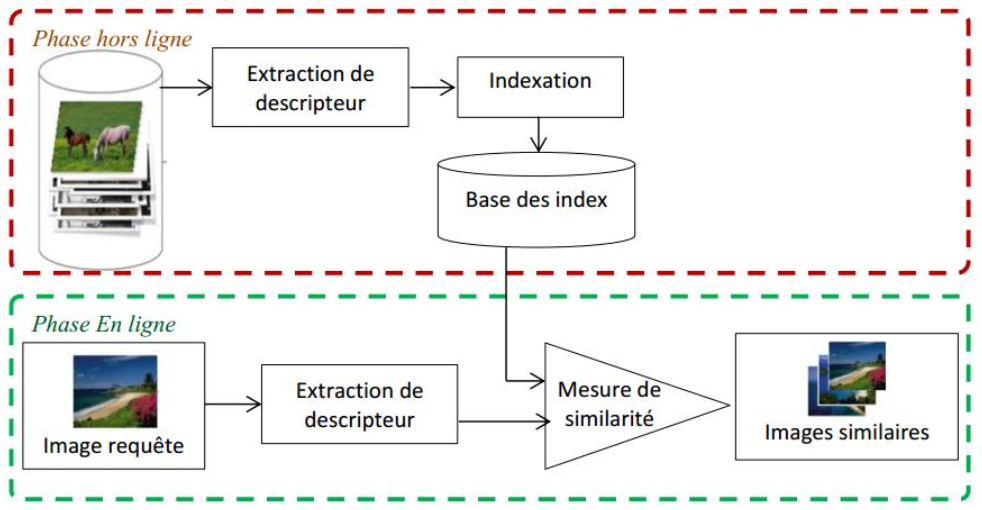
\includegraphics[width=0.65\textwidth]{Figures/cbir_principe} % Include the image .png
		\caption{ Schéma général d’un CBIR.}
\end{figure}

Lors de la phase d'indexation, le calcul de descripteur consiste en l'extraction de caractéristiques visuelles des images telles que:
\begin{itemize}
	\item la texture (filtre de Gabor, transformée en ondelettes discrète…)
	\item la couleur (la segmentation, les points d’intérêts, les régions d’intérêts,
	histogramme de couleurs, histogrammes dans l'espace RGB ou dans TSV, …),
	\item les formes (descripteurs de Fourier,Zernik, ART…),
	\item une combinaison de plusieurs de ces caractéristiques.
\end{itemize}

Ces caractéristiques sont dites de bas-niveau, car elles sont très proches du contenu signal (pixel), et ne véhiculent pas de sémantique particulière sur l'image.\\

Une fois ces caractéristiques extraites, la comparaison consiste généralement à définir diverses distances entre ces caractéristiques, et de définir une mesure de similarité globale
entre deux images. Au moyen de cette mesure de similarité et d'une image requête, on peut alors calculer l'ensemble des mesures de similarités entre cette image requête et l'ensemble des images de la base d'images. On peut alors ordonner les images de la base suivant leur score, et présenter le résultat à l'utilisateur, les images de plus grand score étant considérées comme les plus similaires.\\

Ce genre de système ne nécessite pas forcément une image requête pour rechercher d'autres images. Par exemple, il est possible de rechercher des images plutôt bleues, ou alors de dessiner une forme et demander de chercher toutes les images qui possèdent un objet de forme similaire.



Une des étapes essentielles en analyse d'images par le contenu est l'extraction d'une description de bas niveau de l’image. Cette description est une représentation numérique (analyse statistique, analyse quantitative, ...) des caractéristiques visuelles de l'image, généralement sous la forme d’un vecteur ou d’un ensemble de vecteurs.
Cette description doit avoir deux caractéristiques importantes :
\begin{itemize}
	\item elle doit conserver suffisamment d’information pour être discriminante, c’est-à-dire différencier deux images avec un contenu visuel différent;
	\item elle doit être la plus invariante possible (aux bruits; aux variations d’échelle; aux variations de contraste; aux déformations; etc) pour pouvoir généraliser le contenu visuel d’une image à une autre image qui n’est pas identique.
\end{itemize}


Nous présentons dans la suite les différentes familles de descripteurs.


\subsection{Descripteur globaux et descripteurs locaux}
On peut résumer l’ensemble des informations visuelles de l’image en un unique descripteur
global, ou plusieurs descripteurs locaux caractérisant chacun une partie de l’image. Les
techniques modernes en imagerie tendent à privilégier les descripteurs locaux aux globaux car
les descripteurs locaux sont plus efficaces et ils permettent une recherche plus fine et
absorbent mieux certaines variations.

\subsubsection{Descripteurs globaux}
Dans le cas de descripteurs globaux, un seule descripteur décrit la totalité de l’image, cela
les rend robustes au bruit qui peut affecter le signal, les histogrammes de couleur et des
niveaux de gris en sont des exemples classiques [Stricker 94]. De nombreux descripteurs
globaux sont également basés sur la texture et la couleur. La couleur aussi fait partie des
premières primitives visuelles utilisées. Le plus simple des descripteurs globaux basés sur la
couleur consiste à construire l’histogramme des couleurs.
L’inconvénient de ces descripteurs est qu’ils ne permettent pas de distinguer des parties de
l’image, ils ne distinguent pas, par exemple, les objets dans l’image, sauf dans le cas où
l’image ne contient qu’un seule objet sur un fond uni.

\subsubsection{Descripteurs locaux}
Les descripteurs locaux s’associent à une partie/région de l’image qu’on commence par
détecter avant de calculer le descripteur, cette partie peut concerner un objet par exemple, la
détection se fait indépendamment de la position dans l’image, ce qui assure l’invariance par
translation, rotation, etc .

Les descripteurs locaux sont de nos jours les caractéristiques visuelles les plus couramment
utilisées en analyse d’image par le contenu. Ils permettent de décrire l’ensemble des
informations visuelles d’une région de l’image en un descripteur (vecteur). La région
d’extraction est appelée région d’intérêt et elle est généralement centrée sur un point d’intérêt
Les descripteurs locaux ont une très bonne capacité de discrimination pour déterminer si
deux régions sont similaires ou dissimilaires. Cela les rends particulièrement utiles en vision
par ordinateur, notamment pour de la mise en correspondance de points d’intérêts. Ils sont
utilisés en : odométrie visuelle [Nistér 04] ; reconstruction 3D [Mouragnon 06] ; détection
d’objets [Lowe 99] ; recherche d’images par le contenu [Perronnin 10], [Negrel 14] ; etc.
Dans le chapitre suivant, nous présentons un descripteur local basé sur la segmentation par
k-means.

\subsection{Combinaison des descripteurs}

Les attributs: couleur, texture, forme décrivent les images par leur contenu visuel. La
combinaison de ces attributs peut être mieux caractérisée le contenu. Il est donc intéressant de
combiner ces différents attributs pour une recherche plus efficace et plus discriminante. Les
problèmes qui se posent lors de la combinaison de ces différents attributs pour la recherche et
l’indexation sont au moins de trois ordres :
\begin{itemize}
	\item L'espace de description : Le choix de l'espace de description consiste à rechercher les
	attributs visuels significatifs de la base de données d'images, l'ensemble de ces
	attributs étant représenté par un nuage de points dans un espace dimensionnel haut,
	alors les vecteurs contiennent plusieurs attributs, un problème qui se pose est celui de
	la dimension de l'espace de description. Ce problème est connu dans la communauté
	des bases de données par la malédiction de la dimension, lorsque le nombre de
	dimensions augmente, le volume de l'espace croît rapidement si bien que les données
	se retrouvent « isolées » et deviennent éparses.
	\item La mesure de la similarité : Il s'agit d'une étape essentielle dans tout système de
	recherche. Dans le cas où les images sont décrites par différents attributs, une solution
	classique pour mesurer la similarité est de calculer séparément les mesures de
	similarité pour chaque attribut et de déduire ensuite une mesure composite de la
	similarité globale entre les images. Cela suppose évidemment que les différents
	attributs sont indexés séparément (avec des structures d'index séparées). Dans la base de données, il y a peu de méthodes qui utilisent plusieurs index pour structurer les
	données. Une autre difficulté liée à la similitude est de déterminer comment combiner
	plusieurs mesures souvent définies sur des domaines différents, avec des dynamiques
	différentes, des degrés d'importance différents, surtout pour l'utilisateur, mais aussi de
	natures différentes.
	\item Structuration : la phase de construction d'une structure d'index est une étape utile dans
	le cas où les données sont volumineuses et appartiennent à un grand espace de
	description. Il s'agit de structurer les nuages de points relatifs aux descripteurs des
	images et de les stocker efficacement dans une machine. Cette tâche de structuration
	peut s'avérer difficile dans le cas où les données à structurer sont de nature hétérogène.
	La difficulté réside dans le choix de la distance à utiliser pour structurer (mise en place
	d'un index) et dans la standardisation des différents types de données.
\end{itemize}


\subsubsection{Espace des couleurs}
Une couleur est généralement représentée par trois composantes. Ces composantes définissent un espace des couleurs. On peut citer l'espace RVB, l'espace CIE (Commission Internationale de l'Eclairage) XYZ ou Yxy, ou encore l'espace Lab. Selon l'espace de couleurs choisi pour représenter une image couleur, le nuage des couleurs (c'est à dire l'ensemble des couleurs de l'image) n'aura pas la même répartition dans l'espace 3D.

\begin{figure}[H]
	\label{fig:espaceRVB}
	\centering
	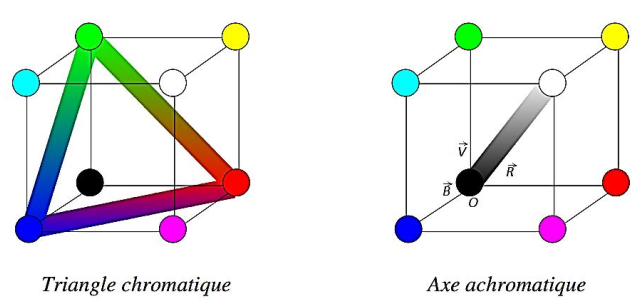
\includegraphics[width=0.65\textwidth]{Figures/espaceRVB} % Include the image .png
	
	\caption{Espace de couleur RVB.}
	
\end{figure}

Les espaces de couleurs classiques, tels que le RVB, CIE XYZ, ...etc, sont issus d'une approche purement physique, sans la prise en compte de données psychophysiques. Dans d'autre espaces de couleur, tels que l'espace Lab, l'approche physique est corrigée selon des données de la vision humaine.\\

De nombreuses méthodes de descriptions d'images proposent de caractériser la couleur dans certains espaces couleurs pour profiter des propriétés de ces derniers. La figure 1.6
montre les principaux espaces couleurs utilisés en indexation d’images.

\begin{figure}[H]
	\label{fig:espaceCouleur}
	\centering
	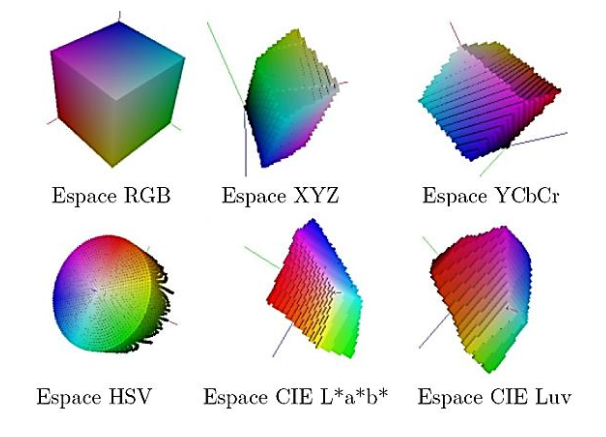
\includegraphics[width=0.45\textwidth]{Figures/espaceCouleur} % Include the image .png
	\caption{Les principaux espaces couleurs utilisés en indexation d’images.}
	
\end{figure}

On peut principalement citer :
\begin{itemize}
	\item \textbf{RGB} (Rouge, Vert, Bleu): est le plus utilisé car la plupart des images originelles sont codées dans cet espace couleur, ce qui ne nécessite pas de transformation inter
	espace couleur, donc facilement applicable.
	
	\item \textbf{HSV}: chaque composante représente respectivement la teinte, la saturation et la luminance.
	
	\item \textbf{YCbCr}: est utilisé dans les normes MPEG 1, 2 et 4, ses composantes sont décorrélées et de faibles dynamiques, ce qui permet de bons taux de compression.
	
	\item \textbf{L*a*b*} ou \textbf{CIE Luv}: sont des espaces couleurs perceptuellement uniformes. Ces espaces ont été créés dans le but de rendre plus homogène l’espace des couleurs et de
	permettre de mesurer uniformément les distances entre couleurs en tout point de l'espace. Deux couleurs proches dans ces espaces couleurs sont proches perceptuellement. Ces espaces sont grandement utilisés dans les systèmes de comparaison d'images.
\end{itemize}
%----------------------------------------------------------------------------------------
%	SECTION 2
%----------------------------------------------------------------------------------------


\section{Conclusion}
Ce chapitre a fait l’état de l’art sans exhaustivité des différents descripteurs des attributs
visuels pouvant être utilisés pour la recherche d’images par le contenu ainsi que les approches
correspondantes. Aussi, nous avons dressé une liste des types de descripteurs et les mesures
de similarités avec leurs avantages et leurs inconvénients. Le chapitre suivant se focalisera sur
notre solution détaillée, le schéma de CBIR, les techniques d’extraction de descripteur. Le
choix d’un meilleur descripteur et d’une mesure de similarité promet une bonne pertinence
d’un système CBIR.